\documentclass[sigconf]{acmart}
\usepackage{amsmath}
\usepackage{graphicx}
\usepackage{booktabs}
\usepackage{seqsplit}
\usepackage{tikz}
\usetikzlibrary{arrows.meta,positioning,decorations.pathreplacing}
\DeclareRobustCommand{\pathtt}[1]{\texttt{\seqsplit{#1}}}

\AtBeginDocument{%
  \providecommand\BibTeX{{%
    Bib\TeX}}}

\setcopyright{none}
\settopmatter{printacmref=false, printccs=false, printfolios=true}
\renewcommand\footnotetextcopyrightpermission[1]{}

\title{Legible Is Not Controllable: A Frozen Reality Check for Prompt-vs-Latent Behavioral Control in LLMs}

\author{Anonymous Authors}
\affiliation{%
  \institution{Anonymous Institution}
  \country{}}
\email{anonymous@example.com}

\begin{document}


\begin{abstract}
Interfaces that make large language models more legible often invite a stronger promise: if users can name or visualize a cognitive axis, perhaps they can steer behavior by moving along the same latent direction. We test that promise as a reality check rather than as a new steering method. Motivated by internal non-surjectivity as background \cite{mishra2026nonsurj}, we separate representational readability from behavioral control. First, an exploratory measurement finds a representational facade for several metacognitive axes in Qwen2.5-7B: readable prompts occupy only part of the corresponding extracted activation direction. We then use a frozen, fairness-controlled, independently audited DEV/TEST adjudicator to compare bounded best-prompt control with naive off-the-shelf CAA and ITI steering across Qwen2.5-7B and Llama-3-8B. Across this tested grid, latent steering does not beat the prompt ceiling on the adjudicated axes, and the uncertainty axis consistently harms calibration; see the generated results table and calibration-harm figure. These findings do not imply that all steering fails, especially given trained prompt-mimicking steering \cite{heyman2026steer}. They instead argue for cognitive consoles that surface the limits and failure modes of legible control, helping users recalibrate trust rather than offering a latent ``control slider.''
\end{abstract}

\maketitle

\section{Introduction}
\label{sec:introduction}
A growing class of language-model interfaces asks users to treat model behavior as something they can inspect, name, and adjust. Prompt instruments reify natural-language commands as manipulable interface objects; transparency work asks how non-experts should understand model capabilities and uncertainty; feature-steering interfaces suggest that latent directions may become usable controls \cite{riche2025aiinstr,liao2024transparency,huang2025steering}. These systems respond to a real HCI need. When people use generative AI for reasoning, search, drafting, or decision support, they are not only asking for an output. They are also trying to monitor whether the model is being careful, skeptical, calibrated, or merely fluent \cite{tankelevitch2024metacog}.

The hard question is whether a readable axis is also a safe control primitive. A latent direction can look meaningful to an analyst: it can separate contrastive prompts, align with an interpretable label, or move generated text in a recognizable way. But user-facing control requires more than recognizability. It requires that acting along the direction improves the behavior that matters, under a fair comparison to what a user could already do with prompts. For a cognitive console, the distinction is not semantic bookkeeping. If a console turns a legible direction into a slider, users may infer that reading the model's state and steering the model's behavior are two sides of the same instrument. Our thesis is that this inference can be false: a cognitive axis can be legible in representations yet fail as a behavioral control, and naive latent steering can even make calibration worse.

Prior theory gives a reason to be suspicious, but not a result we can simply import. Mishra et al. show internal non-surjectivity: activation steering can reach residual states that bounded prompting does not reproduce \cite{mishra2026nonsurj}. We use that workshop result as motivation for a prompt/latent gap at the internal-state level. It does not, by itself, prove that prompting and steering diverge on user-visible behavior. Conversely, the strongest counterpoint is not hypothetical. Prompt-steering-recovery work shows that trained steering can mimic prompting \cite{heyman2026steer}. Our claim is therefore deliberately narrow: it concerns bounded prompt effort versus naive, off-the-shelf CAA and ITI steering on metacognitive axes for the two tested model families. It is not an impossibility theorem for latent control.

We make this narrow claim through a frozen behavioral adjudication rather than an anecdotal steering demo. The protocol selects both the best prompt and the steering strength on DEV, evaluates on disjoint TEST items, compares paired item-level outcomes, controls multiplicity across axes, and applies a coherence gate before crediting a latent win. The comparison is designed to answer the reviewer question that matters for an interface: if a non-expert already has a bounded prompt channel, does an interpretable latent direction add behavioral control on top of that channel? The answer in our tested setting is a qualified but consequential no. Across the full CAA/ITI by Qwen/Llama grid, latent steering does not exceed the bounded best-prompt ceiling on the adjudicated axes, and the calibration-harm finding on uncertainty replicates across the grid. A concurrent study by Sprejer et al. reaches a related degradation pattern with different machinery, using SAE features and MMLU rather than our pre-registered CAA/ITI behavioral adjudication \cite{sprejer2026mindgap}. We treat that work as external corroboration, not as a scoop.

This negative result is useful because it changes what a console should promise. The design implication is not that latent methods are useless, nor that users should be denied model-state information. It is that an HCI system should instrument the boundary between legibility and control. A console can show where a direction is readable, where it fails to transfer to behavior, where calibration is harmed, and where stronger or trained steering would need a separate frozen test. Such a console supports trust recalibration: it helps users learn when a legible model state is diagnostic evidence and when it is not a control affordance.

This paper contributes:
\begin{enumerate}
  \item \textbf{An exploratory representational measurement.} We measure a representational-facade pattern on Qwen2.5-7B metacognitive axes, showing that readable prompts can occupy only part of an extracted axis direction. This claim is explicitly exploratory and single-family pending replication.
  \item \textbf{A frozen prompt-vs-latent behavioral adjudication.} We provide a pre-registered, fairness-controlled, independently audited comparison of bounded best-prompt control against naive CAA/ITI steering across the tested Qwen/Llama method--model grid.
  \item \textbf{A generalized scoped negative with calibration harm.} Under that adjudicator, naive latent steering fails to beat the bounded prompt ceiling in every tested cell, while uncertainty calibration is harmed; quantitative values are reported only in the generated table and figure.
  \item \textbf{A design stance for cognitive consoles.} We argue that HCI tools should surface limits, failed transfer, and trust-calibration risks rather than presenting legible latent directions as user-facing control sliders. This is a design implication from model evidence, not a user-study claim.

\end{enumerate}

\begin{figure*}[t]
  \centering
  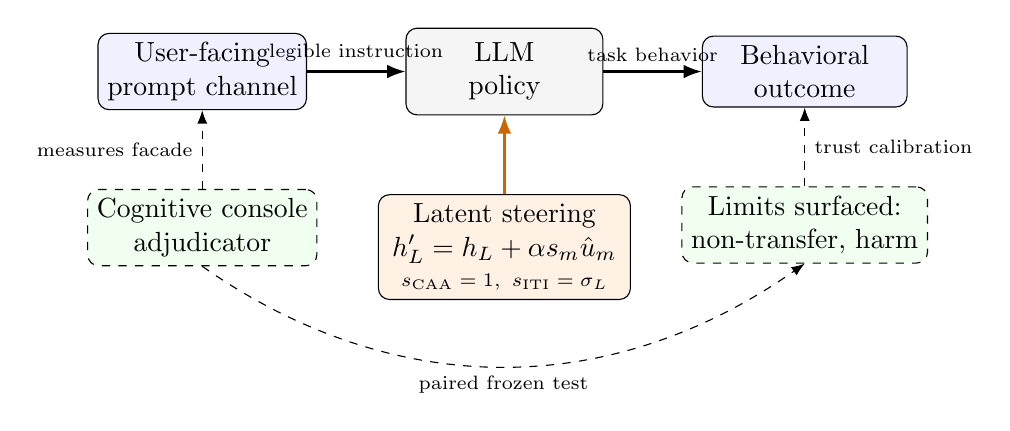
\begin{tikzpicture}[
  >=Latex,
  channel/.style={draw, rounded corners, align=center, minimum width=2.6cm, minimum height=0.8cm, fill=blue!6},
  latent/.style={draw, rounded corners, align=center, minimum width=3.2cm, minimum height=1.05cm, fill=orange!10},
  model/.style={draw, rounded corners, align=center, minimum width=2.5cm, minimum height=1.1cm, fill=gray!8},
  probe/.style={draw, dashed, rounded corners, align=center, minimum width=2.6cm, minimum height=0.8cm, fill=green!6}
]
  \node[channel] (user) {User-facing\\prompt channel};
  \node[model, right=1.25cm of user] (llm) {LLM\\policy};
  \node[channel, right=1.25cm of llm] (behavior) {Behavioral\\outcome};

  \node[latent, below=1.0cm of llm] (latent) {Latent steering\\$h'_L=h_L+\alpha s_m\hat u_m$\\[-1pt]\scriptsize $s_{\rm CAA}=1,\ s_{\rm ITI}=\sigma_L$};
  \node[probe, below=1.0cm of user] (console) {Cognitive console\\adjudicator};
  \node[probe, below=1.0cm of behavior] (limits) {Limits surfaced:\\non-transfer, harm};

  \draw[->, thick] (user) -- node[above, font=\scriptsize]{legible instruction} (llm);
  \draw[->, thick] (llm) -- node[above, font=\scriptsize]{task behavior} (behavior);
  \draw[->, thick, orange!80!black] (latent) -- (llm);
  \draw[->, dashed] (console) -- node[left, font=\scriptsize]{measures facade} (user);
  \draw[->, dashed] (console.south) to[out=-35,in=-145] node[below, font=\scriptsize]{paired frozen test} (limits.south);
  \draw[->, dashed] (limits) -- node[right, font=\scriptsize]{trust calibration} (behavior);
\end{tikzpicture}

  \caption{Dual-channel cognitive-console framing. The prompt channel is user-legible, while the latent-steering channel intervenes on hidden states; the console instruments where legibility fails to transfer to behavioral control. This HCI schematic is conceptual, not a result artifact.}
  \label{fig:concept}
\end{figure*}

\section{Related Work}
\label{sec:related-work}

\subsection{Non-surjectivity and Prompt--Latent Mismatch}
Our work starts from a gap between two meanings of control. In the prompt channel, a user expresses an intention in natural language and observes the resulting behavior. In the latent channel, an analyst or system intervenes on internal representations. Mishra et al. provide the theoretical background for why these channels need not coincide: steered residual activations can be internally non-surjective with respect to bounded prompts \cite{mishra2026nonsurj}. We do not treat that workshop result as our empirical finding. Instead, we ask whether a related gap appears at the behavioral level, under a frozen comparison between the best available bounded prompt and naive latent steering.

The main counterpoint is prompt-steering recovery. Heyman and Vandeputte show that trained steering can mimic prompting \cite{heyman2026steer}. That result sharply limits any broad reading of our negative finding. We therefore scope our contribution to off-the-shelf CAA and ITI, not to learned or optimized steering methods. The planned latent-recovery arm is the direct response: if a trained steering procedure recovers prompt behavior under the same adjudicator, it would not invalidate our frozen negative result for naive steering, but it would identify a different class of latent control.

\subsection{Activation Steering Lineage}
Activation steering has developed a rich toolkit for turning representational directions into interventions. Contrastive Activation Addition constructs mean-difference directions from paired examples and adds them during inference \cite{rimsky2024caa}. Inference-Time Intervention uses probe-derived directions to alter truthful-answer behavior \cite{li2023iti}. Activation addition and representation engineering broaden this family of techniques and motivate the idea that interpretable latent coordinates can be operationalized as controls \cite{turner2023actadd,zou2023repe}. Instruction-steering work is especially close because it links natural-language instructions to activation directions \cite{stolfo2025instr}.

Our experiment does not dispute that these interventions can change outputs. It asks a stricter interface question: when the comparator is the best bounded prompt selected under the same DEV/TEST discipline, does the latent intervention improve the target behavior without degrading usable output? Recent work on steerability limits and safety failures similarly cautions that latent interventions can be brittle, context-dependent, or harmful \cite{fan2026asteer,korznikov2025rogue}. Sprejer et al. independently report capability--behavior trade-offs when steering SAE features \cite{sprejer2026mindgap}. Their method, tasks, and registration status differ from ours, which is why we frame their result as corroborating evidence for the broader risk rather than as the same contribution.

\subsection{HCI, Transparency, and Trust Neighbors}
HCI research has long treated AI interaction as a problem of legibility, control, and calibrated reliance. Work on metacognitive demands in generative AI explains why users need to monitor not only what a model says but how confidently or carefully it appears to reason \cite{tankelevitch2024metacog}. Human-centered transparency roadmaps argue that explanations and controls must be designed around what users can act on, not merely what systems can expose \cite{liao2024transparency}. Studies of system prompts, instruction conflicts, and confidence-signal recalibration further show that users negotiate control across visible and hidden layers of AI behavior \cite{neumann2026whocontrols,he2025coninstruct,li2026learntrust}.

Several interface neighbors make parts of the same design space concrete. AI-Instruments reifies prompt-layer actions, but does not introduce a latent channel \cite{riche2025aiinstr}. Huang and Lim study layperson interfaces for SAE feature steering and persona building, a strong HCI neighbor to our console framing \cite{huang2025steering}. Labarta et al. present a human-centered activation-steering workflow for vision/CLIP expert debugging rather than LLM generation \cite{labarta2026attribution}. Latent Manipulator steers embedding visualizations rather than model behavior \cite{raval2026latman}. Work connecting latent space, steering vectors, calibration, and trust shows that the phrase ``latent control'' is already crowded, but does not supply a prompt-vs-latent behavioral adjudication for metacognitive axes \cite{subramani2026latent}. Our distinctive move is to make the prompt channel and the latent channel compete under a frozen behavioral test, then translate the resulting boundary into a console design stance.

\subsection{Nearest-Neighbor Novelty Contrast}
\label{sec:novelty-contrast}
Table~\ref{tab:novelty-neighbors} summarizes the nearest neighbors. The contrast is intentionally methodological rather than rhetorical: the paper's distinct unit is a frozen, pre-registered, fairness-controlled prompt-vs-naive-latent adjudication across the tested method--model grid, tied to an HCI legibility-console framing. The machine-readable provenance is in \pathtt{docs/paper/citation-map.yaml}.

\begin{table*}[t]
  \centering
  \caption{Nearest-neighbor novelty contrast. The paper's distinct unit is a frozen, pre-registered, fairness-controlled prompt-vs-naive-latent adjudication across 2 methods $\times$ 2 models on metacognitive axes, tied to an HCI legibility-console framing.}
  \label{tab:novelty-neighbors}
  \begin{tabular}{p{0.25\linewidth}p{0.32\linewidth}p{0.35\linewidth}}
    \toprule
    Prior work & What they test & What we uniquely adjudicate \\
    \midrule
    Sprejer et al. \cite{sprejer2026mindgap} & Closest empirical neighbor: feature steering can create capability--behavior trade-offs and degradation relative to prompting. & External corroboration for C2/calibration-harm, not a scoop: they use Goodfire SAE features rather than CAA/ITI, evaluate MMLU rather than metacognitive axes, and do not use a frozen pre-registration, 2$\times$2 method--model grid, or HCI legibility-console framing. \\
    Mishra et al. \cite{mishra2026nonsurj} & Internal residual-state non-surjectivity under activation steering. & Behavioral prompt-vs-latent transfer under frozen DEV/TEST adjudication; Mishra is workshop background/motivation only. \\
    Heyman and Vandeputte \cite{heyman2026steer} & Trained steering that mimics prompting. & Our result is deliberately about naive/off-the-shelf CAA/ITI under bounded prompt effort; PSR motivates the planned latent-recovery arm. \\
    Rimsky et al. and Li et al. \cite{rimsky2024caa,li2023iti} & Steering methods: CAA and ITI. & We test whether those legible directions beat the best prompt on task outcomes with fairness controls and hostile audits. \\
    Fan et al.; Korznikov et al. \cite{fan2026asteer,korznikov2025rogue} & Steerability limits and safety-domain failures of activation steering. & We provide a metacognitive, prompt-vs-latent, pre-registered behavioral adjudication rather than a broad steering benchmark or safety attack. \\
    Huang and Lim \cite{huang2025steering} & Layperson GUI for SAE feature steering/persona building. & No human-study claim here; our pure-model contribution is prompt-vs-latent behavioral non-transfer and its design implication. \\
    Riche et al.; Labarta et al.; Raval et al. \cite{riche2025aiinstr,labarta2026attribution,raval2026latman} & Prompt instruments, expert vision/CLIP activation steering, and embedding-visualization manipulation. & We focus on LLM behavioral control and calibration harm; Labarta is vision/CLIP and Latent Manipulator steers visualizations, not LLM generations. \\
    \bottomrule
  \end{tabular}
\end{table*}

\section{Methods}
\label{sec:methods}

\subsection{C1 Facade Measurement}
The C1 figure is rebuilt from \pathtt{results/gpu\_7b\_2026-07-23/c1/c1\_facade\_results.json}; provenance is recorded in \pathtt{docs/paper/figure-manifests/c1-ratio-ci.yaml}. No numeric values are copied manually into this file. For each axis, the script plots the frozen artifact's scale-free facade ratio
\begin{equation}
  r_a = \frac{\mathrm{prompt\_reach}_a}{\mathrm{pole\_reach}_a},
  \label{eq:facade-ratio}
\end{equation}
and the random-null reference on the same scale, $\mathrm{pole\_null\_p95}_a /\allowbreak \mathrm{pole\_reach}_a$. This measurement is exploratory and Qwen2.5-7B only.

\subsection{Frozen Behavioral Adjudicator}
The adjudicator uses DEV-only selection of prompts and steering strengths, paired TEST comparisons, item-cluster bootstrap, Bonferroni correction, and a coherence gate. The protocol source is \pathtt{docs/ledgers/prereg-c2b-adjudication.md}. CAA constructs a mean-difference steering vector
\begin{equation}
  v = \mathbb{E}_{x \in A^+}[h_L(x)] - \mathbb{E}_{x \in A^-}[h_L(x)],
  \qquad
  h'_L = h_L + \alpha \hat{v},
  \label{eq:caa-steering}
\end{equation}
where $L$ is the intervention layer and $\hat{v}$ is the unit direction. ITI uses the same intervention form with a probe-derived direction.

For each TEST item $i$, the frozen rule compares steer-only behavior against the DEV-selected best prompt using the paired difference
\begin{equation}
  d_i = \mathrm{steer}_i - \mathrm{prompt}_i.
  \label{eq:paired-diff}
\end{equation}
The confidence interval is obtained by paired item-cluster bootstrap: resample items as clusters, each carrying its $k$ samples, with $B \ge 10000$. For the three adjudicated axes, the per-axis CI is the Bonferroni two-sided interval at
\begin{equation}
  1 - \frac{0.05}{3} = 0.98333.
  \label{eq:bonferroni-ci}
\end{equation}
An axis passes iff
\begin{equation}
  \begin{aligned}
    0 &\notin \mathrm{CI}_{0.98333}(\bar d_a) \\
    &\wedge\quad \bar d_a \ge \delta \\
    &\wedge\quad \mathrm{coherence\ ratio}_a \le 1.5,
    \qquad \delta = 0.05.
  \end{aligned}
  \label{eq:axis-pass}
\end{equation}
The frozen verdict is STRONG\_GO for at least two passing axes, CONDITIONAL\_GO for exactly one passing axis, and KILL\_PLAN\_D for zero passing axes. Outcome definitions are fixed as deliberation = accuracy, skepticism = false-premise rejection rate, and uncertainty = $1-\mathrm{Brier}$ (Table~\ref{tab:axis-outcomes}).
\begin{table}[t]
  \centering
  \caption{Behavioral outcome definitions for deliberation, skepticism, and uncertainty.}
  \label{tab:axis-outcomes}
  \begin{tabular}{ll}
    \toprule
    Axis & Outcome definition \\
    \midrule
    Deliberation & Accuracy \\
    Skepticism & False-premise rejection rate \\
    Uncertainty & $1 - \mathrm{Brier} = 1 - (\mathrm{conf}_i - \mathrm{correct}_i)^2$ \\
    \bottomrule
  \end{tabular}
\end{table}


\subsection{Steering Families and Models}
The 2$\times$2 robustness arm covers CAA/ITI $\times$ Qwen2.5-7B/Llama-3-8B. Llama provenance follows D-0038.

\subsection{Audit and Artifact Lineage}
All main tables and figures must trace to manifests under \pathtt{docs/paper/table-manifests/} and \pathtt{docs/paper/figure-manifests/}. The LaTeX source includes generated figures and table inputs whose numeric values are rebuilt from frozen artifacts, not hand-entered.

\section{Results}
\label{sec:results}

\subsection{Representational Facade Ratio (C1)}
\begin{figure}[t]
  \centering
  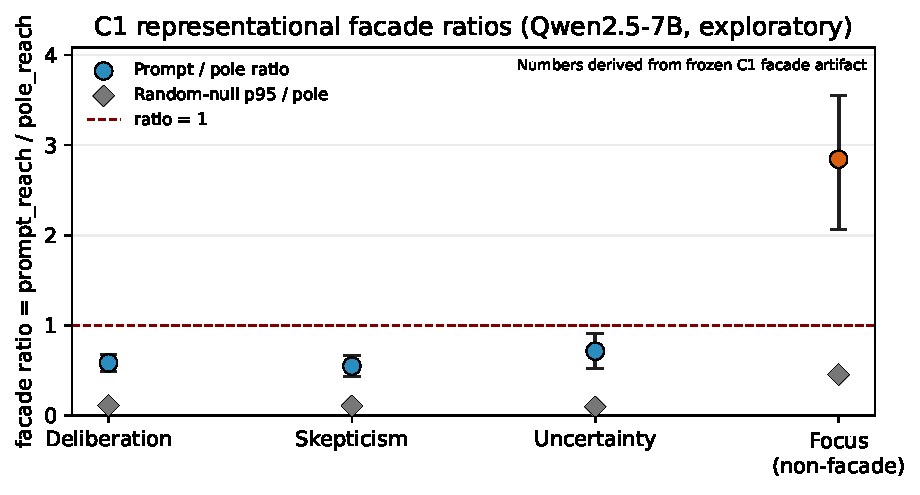
\includegraphics[width=\linewidth]{figures/c1-ratio-ci.pdf}
  \caption{Exploratory representational-facade ratios by axis for Claim C1, generated from experiment \pathtt{c1-facade-d710b4b4-0001} (\pathtt{results/gpu\_7b\_2026-07-23/c1/c1\_facade\_results.json}). Focus is labeled as non-facade/overshoot; C1 remains single-model exploratory evidence.}
  \label{fig:c1-ratio-ci}
\end{figure}

Figure~\ref{fig:c1-ratio-ci} carries C1 with explicit caveats: focus overshoot/no-facade, deliberation layer sensitivity, and pending Llama replication.

\subsection{Frozen Prompt-vs-Latent Delta Table (C2)}
% Auto-generated by docs/paper/scripts/make_c2_delta_table.py from frozen JSON artifacts.
\begin{table*}[t]
  \centering
  \caption{Frozen prompt-vs-latent behavioral adjudication across CAA/ITI $\times$ Qwen/Llama. The table supports Claim C2 and is generated from frozen robustness-arm artifacts; CAA$\times$Qwen reproduces the original Qwen adjudication. $\Delta$ is TEST paired steer--prompt outcome; intervals are Bonferroni two-sided CIs at level 0.98333; the pre-registered meaningful margin is $\delta=0.05$.}
  \label{tab:c2-delta-4cell}
  \scriptsize
  \begin{tabular}{lllrrrll}
    \toprule
    Method & Model & Axis & $N_{dev}$ & $N_{test}$ & $\alpha$ & $\Delta$ [CI] & Gate / pass \\
    \midrule
    CAA & Qwen2.5-7B & Deliberation & 20 & 40 & 2 & +0.015 [-0.040, +0.070] & ok / fail \\
    CAA & Qwen2.5-7B & Skepticism & 20 & 40 & 6 & -0.080 [-0.225, +0.045] & ok / fail \\
    CAA & Qwen2.5-7B & Uncertainty & 27 & 53 & 8 & -0.228 [-0.370, -0.092] & ok / fail \\
    \addlinespace
    CAA & Llama-3-8B & Deliberation & 20 & 40 & 4 & +0.025 [-0.030, +0.075] & ok / fail \\
    CAA & Llama-3-8B & Skepticism & 20 & 40 & 2 & +0.000 [-0.190, +0.200] & ok / fail \\
    CAA & Llama-3-8B & Uncertainty & 27 & 53 & 8 & -0.072 [-0.103, -0.034] & ok / fail \\
    \addlinespace
    ITI & Qwen2.5-7B & Deliberation & 20 & 40 & 4 & +0.020 [+0.000, +0.055] & ok / fail \\
    ITI & Qwen2.5-7B & Skepticism & 20 & 40 & 2 & -0.100 [-0.270, +0.060] & ok / fail \\
    ITI & Qwen2.5-7B & Uncertainty & 27 & 53 & 12 & -0.103 [-0.136, -0.069] & ok / fail \\
    \addlinespace
    ITI & Llama-3-8B & Deliberation & 20 & 40 & 2 & +0.015 [-0.040, +0.060] & ok / fail \\
    ITI & Llama-3-8B & Skepticism & 20 & 40 & 2 & +0.000 [-0.195, +0.205] & ok / fail \\
    ITI & Llama-3-8B & Uncertainty & 27 & 53 & 6 & -0.084 [-0.115, -0.049] & ok / fail \\
    \bottomrule
  \end{tabular}
  \par\smallskip\raggedright\scriptsize\emph{Notes.} Pass/fail is computed from the unrounded frozen JSON. Displayed means and intervals are rounded to three decimals; a fail can therefore have a small positive displayed estimate or boundary. A pass requires an unrounded CI excluding 0, mean $\ge \delta=0.05$, and the coherence gate to pass, so ITI$\times$Qwen deliberation remains fail because its mean is below $\delta$. The DEV-selected best prompt for each axis/model is identified by its artifact-registry ID; full prompt text is provided in the supplementary manifest (\texttt{c2-delta-4cell.yaml}).
\end{table*}


Table~\ref{tab:c2-delta-4cell} is the C2 headline artifact: all four cells are 0/3 axes under the frozen rule, and all table values are generated by the artifact pipeline.

\subsection{Calibration Harm Across Four Cells}
\begin{figure}[t]
  \centering
  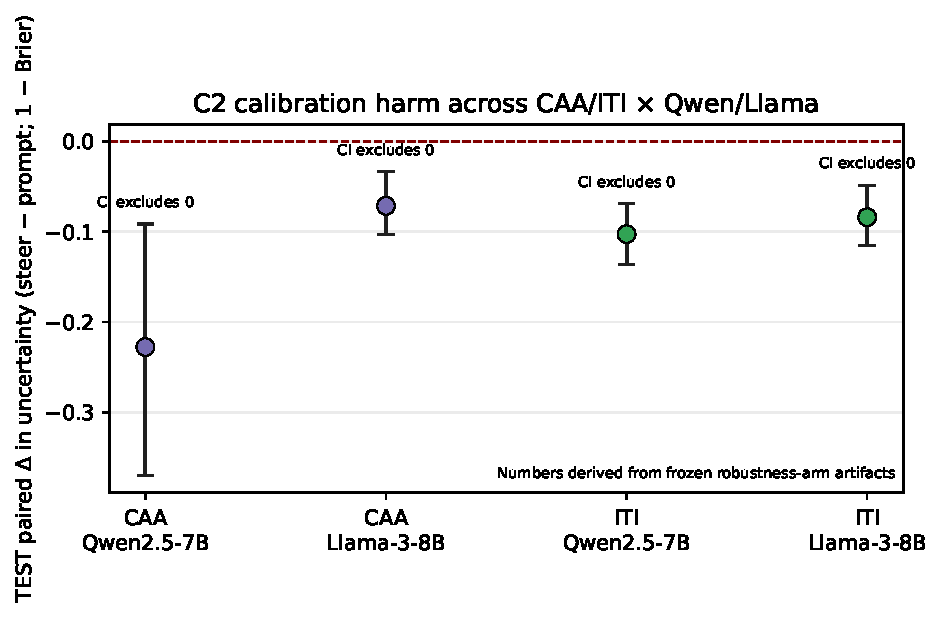
\includegraphics[width=\linewidth]{figures/c2-calibration-harm.pdf}
  \caption{Calibration harm on the uncertainty axis across method--model cells for Claim C2, generated from \pathtt{results/arm\_full/} (E-0006; CAA$\times$Qwen reproduces E-0005). Mechanism remains open after the E-0007 valid null.}
  \label{fig:c2-calibration-harm}
\end{figure}

\section{Design Implications}
\label{sec:design-implications}
\begin{table*}[t]
  \centering
  \caption{Operational failure taxonomy from the methodology asset. This definition table is evidence-tagged, not a result table; it supports the C3 design implication by naming what a console should surface.}
  \label{tab:failure-taxonomy}
  \scriptsize
  \begin{tabular}{L{0.15\linewidth}L{0.25\linewidth}L{0.22\linewidth}L{0.28\linewidth}}
    \toprule
    Class & Observable symptom & Evidence status & Deployment meaning \\
    \midrule
    F1. Legible-but-non-transfer facade & Axis is representationally legible, but steering does not beat best-prompt behavior & Supported in tested scope: E-0003 plus E-0005/E-0006 & Treat latent direction as a diagnostic probe, not production control \\
    F2. Calibration backfire under steering & Uncertainty/calibration axis worsens under steering & Supported/generalized in the tested 2$\times$2: E-0005 and E-0006; mechanism open after E-0007 & Do not deploy naive CAA/ITI steering as a trust-control primitive for calibration-facing products \\
    F3. Coherence-fragility corridor & Higher steering strength risks coherence collapse or forces conservative usable $\alpha$ & Instrumented by preregistered coherence gates; not triggered in tested cells & Stop latent route if coherence deteriorates before meaningful gain \\
    F4. Layer-sensitive instability & Axis effect depends strongly on layer choice & Supported in scope by E-0003 layer sensitivity and E-0006 per-model layer re-derivation & Require layer sweeps and stability checks before deployment \\
    F5. Axis extraction degeneration & Extracted direction overshoots or fails to encode intended construct & Supported in scope by the focus-axis overshoot/no-facade in E-0003 & Exclude the axis from control claims until redesigned \\
    \bottomrule
  \end{tabular}
\end{table*}

C3 is non-empirical on the pure-model route. The design implication is to treat the console as a limits and trust-calibration instrument, not as evidence that users can control latent states. This implication is informed by HCI transparency, metacognition, and trust-calibration work \cite{tankelevitch2024metacog,liao2024transparency,li2026learntrust,neumann2026whocontrols,subramani2026latent}.

\section{Limitations}
\label{sec:limitations}
C1 is exploratory and single-model pending Llama replication. C2 is scoped to bounded prompt effort and naive/off-the-shelf CAA/ITI. The result is not an impossibility theorem, especially given trained steering results \cite{heyman2026steer}. The calibration-harm mechanism is open, and the human-study fork remains owner-gated.

\section{Future Work}
\label{sec:future-work}
Future work includes the frozen latent-recovery arm for PSR-style DEV-optimized steering, Llama C1 replication, a possible owner-approved human study, and a new preregistered mechanism package for calibration harm.

\bibliographystyle{ACM-Reference-Format}
\bibliography{references}

\end{document}
